% chapters/seismo.tex
%
% Copyright 2022 Alexander Lyttle.
%
% This work may be distributed and/or modified under the conditions of the
% LaTeX Project Public License (LPPL) version 1.3 or later.
%
% The latest version of this license is in
% https://www.latex-project.org/lppl.txt and version 1.3 or later is part of
% all distributions of LaTeX version 2005/12/01 or later.
%
%
\chapter[Asteroseismology]{Asteroseismology of Solar-Like Oscillators}

Several decades ago, oscillations of the solar surface were observed, leading to the prediction of waves trapped beneath the solar photosphere \citep{Ulrich1970}. Using the radial velocity method, spectral lines were observed to red and blue shift with a period of around 5 minutes. The study of such oscillations was subsequency called helioseismology \citep{Deubner.Gough1984}. The characterisation and modelling of these oscillations lead to new insight into the solar interior, from understanding rotation \citep{Deubner.Ulrich.ea1979} to the solar neutrino problem \citep{Bahcall.Ulrich1988}.

% \begin{figure}[tbp]
%     \raggedleft
%     \begin{subfigure}[b]{0.25\linewidth}
%         
\includegraphics[width=\linewidth]{figures/spherical_harmonics/0_0.png}
%         \caption*{$l=0,\,m=0$}
%     \end{subfigure}%
%     \begin{subfigure}[b]{0.25\linewidth}
%         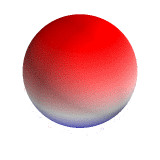
\includegraphics[width=\linewidth]{figures/spherical_harmonics/1_0.png}
%         \caption*{$l=1,\,m=0$}
%     \end{subfigure}%
%     \begin{subfigure}[b]{0.25\linewidth}
%         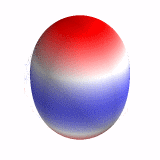
\includegraphics[width=\linewidth]{figures/spherical_harmonics/2_0.png}
%         \caption*{$l=2,\,m=0$}
%     \end{subfigure}%
%     \begin{subfigure}[b]{0.25\linewidth}
%         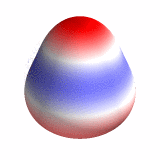
\includegraphics[width=\linewidth]{figures/spherical_harmonics/3_0.png}
%         \caption*{$l=3,\,m=0$}
%     \end{subfigure}%

%     \begin{subfigure}[b]{0.25\linewidth}
%         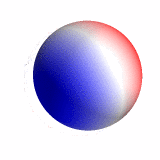
\includegraphics[width=\linewidth]{figures/spherical_harmonics/1_1.png}
%         \caption*{$l=1,\,m=1$}
%     \end{subfigure}%
%     \begin{subfigure}[b]{0.25\linewidth}
%         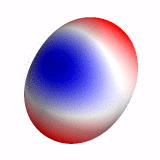
\includegraphics[width=\linewidth]{figures/spherical_harmonics/2_1.png}
%         \caption*{$l=2,\,m=1$}
%     \end{subfigure}%
%     \begin{subfigure}[b]{0.25\linewidth}
%         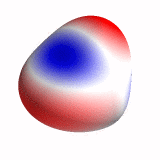
\includegraphics[width=\linewidth]{figures/spherical_harmonics/3_1.png}
%         \caption*{$l=3,\,m=1$}
%     \end{subfigure}%

%     \begin{subfigure}[b]{0.25\linewidth}
%         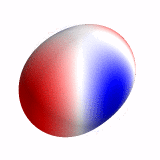
\includegraphics[width=\linewidth]{figures/spherical_harmonics/2_2.png}
%         \caption*{$l=2,\,m=2$}
%     \end{subfigure}%
%     \begin{subfigure}[b]{0.25\linewidth}
%         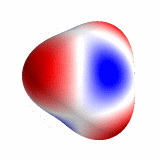
\includegraphics[width=\linewidth]{figures/spherical_harmonics/3_2.png}
%         \caption*{$l=3,\,m=2$}
%     \end{subfigure}%

%     \begin{subfigure}[b]{0.25\linewidth}
%         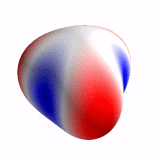
\includegraphics[width=\linewidth]{figures/spherical_harmonics/3_3.png}
%         \caption*{$l=3,\,m=3$}
%     \end{subfigure}
%     \caption{Spherical harmonic modes of oscillation for various combinations of angular degree ($l$) and azimuthal order ($m$).}
%     \label{fig:spherical-harmonics}
% \end{figure}

Damped spherical harmonic oscillator \footnote{The spherical harmonic images were computed using code from \url{https://github.com/warrickball/spherical-harmonics}.}

The fluctuations on the solar surface corresponded to a stochastically driven damped spherical harmonic oscillator. 

% \begin{figure}[tb]
%     \centering
%     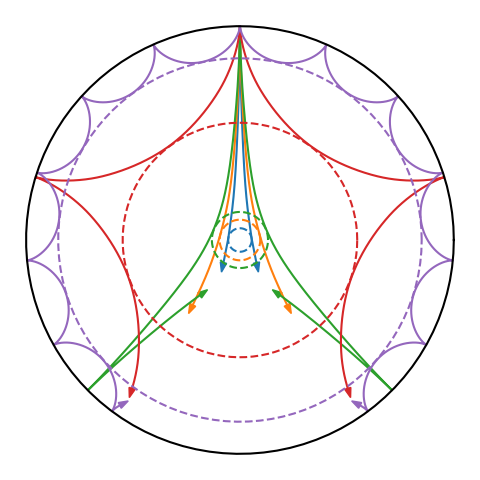
\includegraphics{figures/seismo-wavefronts.png}
%     \caption{The solid lines represent wavefronts of oscillation modes with different angular degree in a two-dimensional star. The dashed lines represent the turning-point of the wave. Lower angular degree modes propagate deeper into the star.}
%     \label{fig:seismo-wavefronts}
% \end{figure}

The oscillations are stochastically excited at the stellar surface. Something about the wave fronts for each mode. How increasing angular degree corresponds to the angle of incidence at the stellar surface. Due to the monotonically increasing sound speed towards the centre of the star, the wavefront bends. We can see the turning points of the wavefronts in Figure \ref{fig:seismo-wavefronts}. Each modes propagation depth allows us to probe different regions of the star. In the case of the Sun, differential rotation. In other stars, low orders only visible.

The limited precision of the radial velocity method meant that observing solar-like oscillations in other stars could be difficult \citep{Christensen-Dalsgaard1982}. However, an alternative method detected solar oscillations by observing brightness fluctuations integrated over the solar surface \citep{Woodard.Hudson1983,Woodard.Hudson1983a}.

Solar-like oscillators are stars which oscillate like the Sun.

\begin{figure}[tb]
    \centering
    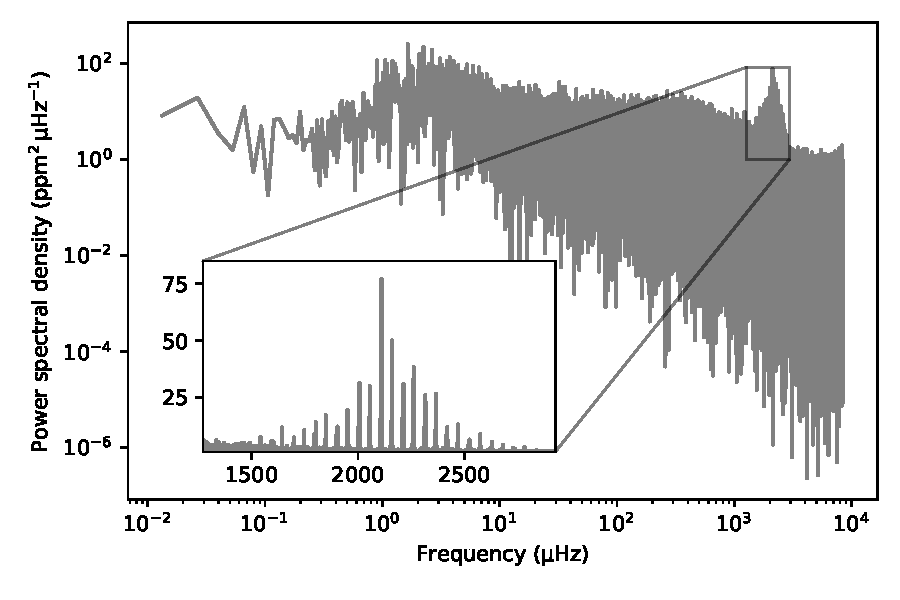
\includegraphics{figures/seismo-psd.pdf}
    \caption{The power spectral density of 16 Cyg A. The inset plot highlights the comb of peaks comprising a Gaussian-like hump in the larger plot.}
    \label{fig:seismo-psd}
\end{figure}

Two well-know solar-like oscillators are in the 16 Cyg binary star system. These bright, main-sequence stars are similar mass to the Sun, and are expected to have a similar outer convective envelope. Figure \ref{fig:seismo-psd}.

The oscillations are solutions to waves trapped in the stellar interior. The solutions, or eigenfrequencies, are unique for \(n, l, m\). \(\nu_{nlm}\). The azimuthal order is visible in a rotating star. For the rest of the chapter, we consider only slowly rotating stars and drop \(m\).

Introduce the asymptotic expression with reference.
%
\begin{equation}
    \nu_{nl} \simeq (n + \frac{l}{2} + \varepsilon) \nu_0,
\end{equation}
%
where,
%
\begin{equation}
    \nu_0 = \left(2 \int_{0}^{R} \frac{\dd r}{c(r)}\right)^{-1}.
\end{equation}
%

The difference between consecutive modes of the same order \(\Delta\nu_{nl} = \nu_{nl} - \nu_{n-1\,l}\). In the same asymptotic limit, we expect \(\Delta\nu_{nl}\) to approximate \(\nu_0\). Therefore, we can reason that some measure of a global \(\Delta\nu\) (e.g. the average \(\langle\Delta\nu_{nl}\rangle\)) can give insight into the mean density of the star.

\begin{figure}[tb]
    \centering
    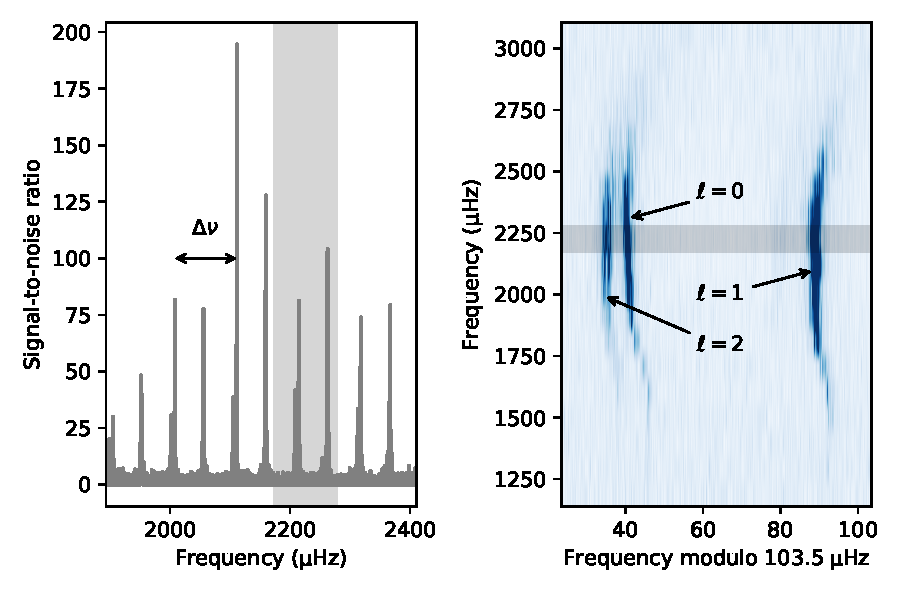
\includegraphics{figures/seismo-echelle.pdf}
    \caption{\emph{Left:} A section of the spectral signal-to-noise ratio (SNR) against frequency for 16 Cyg A. The large frequency spacing (\(\Delta\nu\)) between two radial modes is annotated with a double-headed arrow. The shaded region corresponds to a single row (also highlighted) in the echelle plot (\emph{right}). The echelle plot shows the spectral SNR such that a darker colour represents a higher SNR. Each row spans \SI{103.5}{\micro\hertz} and is stacked in order of frequency. The apparent ridges are labelled according to the angular degree (\(l\)) of the modes they represent.}
    \label{fig:seismo-echelle}
\end{figure}

The comb of peaks in the power spectrum corresponds to oscillation modes in the star. In Figure \ref{fig:seismo-echelle}, we show a small section of the power section with an estimate of the noise divided out. We see a regular repeating pattern, with similar modes repeated by approximately \(\Delta\nu\). If we wrap the spectrum by \(\Delta\nu\), we get the so-called echelle diagram. Ridges of high SNR correspond to modes of different angular degree. From the asymptotic expression, we expect modes of even angular degree grouped together, and likewise for odd angular degrees.

Looking at multiple stars we can see how the peak changes, this is frequency at maximum power. Scales with the acoustic cutoff frequency, so proportional to the surface gravity and effective temperature.

How can asteroseismology tell us about the star? Globally, we can use the scaling relations.

We can also use individual modes and compare with models. Worth noting the surface term here.
